% Options for packages loaded elsewhere
\PassOptionsToPackage{unicode}{hyperref}
\PassOptionsToPackage{hyphens}{url}
\PassOptionsToPackage{dvipsnames,svgnames,x11names}{xcolor}
%
\documentclass[
  letterpaper,
  DIV=11,
  numbers=noendperiod]{scrreprt}

\usepackage{amsmath,amssymb}
\usepackage{iftex}
\ifPDFTeX
  \usepackage[T1]{fontenc}
  \usepackage[utf8]{inputenc}
  \usepackage{textcomp} % provide euro and other symbols
\else % if luatex or xetex
  \usepackage{unicode-math}
  \defaultfontfeatures{Scale=MatchLowercase}
  \defaultfontfeatures[\rmfamily]{Ligatures=TeX,Scale=1}
\fi
\usepackage{lmodern}
\ifPDFTeX\else  
    % xetex/luatex font selection
\fi
% Use upquote if available, for straight quotes in verbatim environments
\IfFileExists{upquote.sty}{\usepackage{upquote}}{}
\IfFileExists{microtype.sty}{% use microtype if available
  \usepackage[]{microtype}
  \UseMicrotypeSet[protrusion]{basicmath} % disable protrusion for tt fonts
}{}
\makeatletter
\@ifundefined{KOMAClassName}{% if non-KOMA class
  \IfFileExists{parskip.sty}{%
    \usepackage{parskip}
  }{% else
    \setlength{\parindent}{0pt}
    \setlength{\parskip}{6pt plus 2pt minus 1pt}}
}{% if KOMA class
  \KOMAoptions{parskip=half}}
\makeatother
\usepackage{xcolor}
\setlength{\emergencystretch}{3em} % prevent overfull lines
\setcounter{secnumdepth}{5}
% Make \paragraph and \subparagraph free-standing
\ifx\paragraph\undefined\else
  \let\oldparagraph\paragraph
  \renewcommand{\paragraph}[1]{\oldparagraph{#1}\mbox{}}
\fi
\ifx\subparagraph\undefined\else
  \let\oldsubparagraph\subparagraph
  \renewcommand{\subparagraph}[1]{\oldsubparagraph{#1}\mbox{}}
\fi

\usepackage{color}
\usepackage{fancyvrb}
\newcommand{\VerbBar}{|}
\newcommand{\VERB}{\Verb[commandchars=\\\{\}]}
\DefineVerbatimEnvironment{Highlighting}{Verbatim}{commandchars=\\\{\}}
% Add ',fontsize=\small' for more characters per line
\usepackage{framed}
\definecolor{shadecolor}{RGB}{241,243,245}
\newenvironment{Shaded}{\begin{snugshade}}{\end{snugshade}}
\newcommand{\AlertTok}[1]{\textcolor[rgb]{0.68,0.00,0.00}{#1}}
\newcommand{\AnnotationTok}[1]{\textcolor[rgb]{0.37,0.37,0.37}{#1}}
\newcommand{\AttributeTok}[1]{\textcolor[rgb]{0.40,0.45,0.13}{#1}}
\newcommand{\BaseNTok}[1]{\textcolor[rgb]{0.68,0.00,0.00}{#1}}
\newcommand{\BuiltInTok}[1]{\textcolor[rgb]{0.00,0.23,0.31}{#1}}
\newcommand{\CharTok}[1]{\textcolor[rgb]{0.13,0.47,0.30}{#1}}
\newcommand{\CommentTok}[1]{\textcolor[rgb]{0.37,0.37,0.37}{#1}}
\newcommand{\CommentVarTok}[1]{\textcolor[rgb]{0.37,0.37,0.37}{\textit{#1}}}
\newcommand{\ConstantTok}[1]{\textcolor[rgb]{0.56,0.35,0.01}{#1}}
\newcommand{\ControlFlowTok}[1]{\textcolor[rgb]{0.00,0.23,0.31}{#1}}
\newcommand{\DataTypeTok}[1]{\textcolor[rgb]{0.68,0.00,0.00}{#1}}
\newcommand{\DecValTok}[1]{\textcolor[rgb]{0.68,0.00,0.00}{#1}}
\newcommand{\DocumentationTok}[1]{\textcolor[rgb]{0.37,0.37,0.37}{\textit{#1}}}
\newcommand{\ErrorTok}[1]{\textcolor[rgb]{0.68,0.00,0.00}{#1}}
\newcommand{\ExtensionTok}[1]{\textcolor[rgb]{0.00,0.23,0.31}{#1}}
\newcommand{\FloatTok}[1]{\textcolor[rgb]{0.68,0.00,0.00}{#1}}
\newcommand{\FunctionTok}[1]{\textcolor[rgb]{0.28,0.35,0.67}{#1}}
\newcommand{\ImportTok}[1]{\textcolor[rgb]{0.00,0.46,0.62}{#1}}
\newcommand{\InformationTok}[1]{\textcolor[rgb]{0.37,0.37,0.37}{#1}}
\newcommand{\KeywordTok}[1]{\textcolor[rgb]{0.00,0.23,0.31}{#1}}
\newcommand{\NormalTok}[1]{\textcolor[rgb]{0.00,0.23,0.31}{#1}}
\newcommand{\OperatorTok}[1]{\textcolor[rgb]{0.37,0.37,0.37}{#1}}
\newcommand{\OtherTok}[1]{\textcolor[rgb]{0.00,0.23,0.31}{#1}}
\newcommand{\PreprocessorTok}[1]{\textcolor[rgb]{0.68,0.00,0.00}{#1}}
\newcommand{\RegionMarkerTok}[1]{\textcolor[rgb]{0.00,0.23,0.31}{#1}}
\newcommand{\SpecialCharTok}[1]{\textcolor[rgb]{0.37,0.37,0.37}{#1}}
\newcommand{\SpecialStringTok}[1]{\textcolor[rgb]{0.13,0.47,0.30}{#1}}
\newcommand{\StringTok}[1]{\textcolor[rgb]{0.13,0.47,0.30}{#1}}
\newcommand{\VariableTok}[1]{\textcolor[rgb]{0.07,0.07,0.07}{#1}}
\newcommand{\VerbatimStringTok}[1]{\textcolor[rgb]{0.13,0.47,0.30}{#1}}
\newcommand{\WarningTok}[1]{\textcolor[rgb]{0.37,0.37,0.37}{\textit{#1}}}

\providecommand{\tightlist}{%
  \setlength{\itemsep}{0pt}\setlength{\parskip}{0pt}}\usepackage{longtable,booktabs,array}
\usepackage{calc} % for calculating minipage widths
% Correct order of tables after \paragraph or \subparagraph
\usepackage{etoolbox}
\makeatletter
\patchcmd\longtable{\par}{\if@noskipsec\mbox{}\fi\par}{}{}
\makeatother
% Allow footnotes in longtable head/foot
\IfFileExists{footnotehyper.sty}{\usepackage{footnotehyper}}{\usepackage{footnote}}
\makesavenoteenv{longtable}
\usepackage{graphicx}
\makeatletter
\def\maxwidth{\ifdim\Gin@nat@width>\linewidth\linewidth\else\Gin@nat@width\fi}
\def\maxheight{\ifdim\Gin@nat@height>\textheight\textheight\else\Gin@nat@height\fi}
\makeatother
% Scale images if necessary, so that they will not overflow the page
% margins by default, and it is still possible to overwrite the defaults
% using explicit options in \includegraphics[width, height, ...]{}
\setkeys{Gin}{width=\maxwidth,height=\maxheight,keepaspectratio}
% Set default figure placement to htbp
\makeatletter
\def\fps@figure{htbp}
\makeatother
\newlength{\cslhangindent}
\setlength{\cslhangindent}{1.5em}
\newlength{\csllabelwidth}
\setlength{\csllabelwidth}{3em}
\newlength{\cslentryspacingunit} % times entry-spacing
\setlength{\cslentryspacingunit}{\parskip}
\newenvironment{CSLReferences}[2] % #1 hanging-ident, #2 entry spacing
 {% don't indent paragraphs
  \setlength{\parindent}{0pt}
  % turn on hanging indent if param 1 is 1
  \ifodd #1
  \let\oldpar\par
  \def\par{\hangindent=\cslhangindent\oldpar}
  \fi
  % set entry spacing
  \setlength{\parskip}{#2\cslentryspacingunit}
 }%
 {}
\usepackage{calc}
\newcommand{\CSLBlock}[1]{#1\hfill\break}
\newcommand{\CSLLeftMargin}[1]{\parbox[t]{\csllabelwidth}{#1}}
\newcommand{\CSLRightInline}[1]{\parbox[t]{\linewidth - \csllabelwidth}{#1}\break}
\newcommand{\CSLIndent}[1]{\hspace{\cslhangindent}#1}

\KOMAoption{captions}{tableheading}
\makeatletter
\makeatother
\makeatletter
\@ifpackageloaded{bookmark}{}{\usepackage{bookmark}}
\makeatother
\makeatletter
\@ifpackageloaded{caption}{}{\usepackage{caption}}
\AtBeginDocument{%
\ifdefined\contentsname
  \renewcommand*\contentsname{Table of contents}
\else
  \newcommand\contentsname{Table of contents}
\fi
\ifdefined\listfigurename
  \renewcommand*\listfigurename{List of Figures}
\else
  \newcommand\listfigurename{List of Figures}
\fi
\ifdefined\listtablename
  \renewcommand*\listtablename{List of Tables}
\else
  \newcommand\listtablename{List of Tables}
\fi
\ifdefined\figurename
  \renewcommand*\figurename{Figure}
\else
  \newcommand\figurename{Figure}
\fi
\ifdefined\tablename
  \renewcommand*\tablename{Table}
\else
  \newcommand\tablename{Table}
\fi
}
\@ifpackageloaded{float}{}{\usepackage{float}}
\floatstyle{ruled}
\@ifundefined{c@chapter}{\newfloat{codelisting}{h}{lop}}{\newfloat{codelisting}{h}{lop}[chapter]}
\floatname{codelisting}{Listing}
\newcommand*\listoflistings{\listof{codelisting}{List of Listings}}
\makeatother
\makeatletter
\@ifpackageloaded{caption}{}{\usepackage{caption}}
\@ifpackageloaded{subcaption}{}{\usepackage{subcaption}}
\makeatother
\makeatletter
\@ifpackageloaded{tcolorbox}{}{\usepackage[skins,breakable]{tcolorbox}}
\makeatother
\makeatletter
\@ifundefined{shadecolor}{\definecolor{shadecolor}{rgb}{.97, .97, .97}}
\makeatother
\makeatletter
\makeatother
\makeatletter
\makeatother
\ifLuaTeX
  \usepackage{selnolig}  % disable illegal ligatures
\fi
\IfFileExists{bookmark.sty}{\usepackage{bookmark}}{\usepackage{hyperref}}
\IfFileExists{xurl.sty}{\usepackage{xurl}}{} % add URL line breaks if available
\urlstyle{same} % disable monospaced font for URLs
\hypersetup{
  pdftitle={FA23-Quantile Regression},
  colorlinks=true,
  linkcolor={blue},
  filecolor={Maroon},
  citecolor={Blue},
  urlcolor={Blue},
  pdfcreator={LaTeX via pandoc}}

\title{FA23-Quantile Regression}
\author{}
\date{2023-10-07}

\begin{document}
\maketitle
\ifdefined\Shaded\renewenvironment{Shaded}{\begin{tcolorbox}[interior hidden, enhanced, breakable, sharp corners, boxrule=0pt, borderline west={3pt}{0pt}{shadecolor}, frame hidden]}{\end{tcolorbox}}\fi

\renewcommand*\contentsname{Table of contents}
{
\hypersetup{linkcolor=}
\setcounter{tocdepth}{2}
\tableofcontents
}
\bookmarksetup{startatroot}

\hypertarget{section}{%
\chapter{}\label{section}}

\bookmarksetup{startatroot}

\hypertarget{introduction}{%
\chapter{Introduction}\label{introduction}}

Quantile regression (QR), like any regression model, illustrates the
relationship between a response variable and one or more predictor
variables. QR differs from traditional regression models, such as
ordinary least squares (OLS) regression, in that it estimates the
conditional \textit{quantiles} of a response variable, given the
predictors' values, as opposed to the conditional \textit{mean} in OLS
regression.

Due to its formula illustrated later, QR has several advantages over
OLS, including relaxed assumptions, efficiency in non-Gaussian
scenarios, and a broader perspective compared to traditional models.
Unlike OLS, QR does not assume the normality of the conditional response
variable distribution and is robust to heteroskedasticity. Furthermore,
by considering the entire conditional distribution, QR offers a
comprehensive understanding of distributions with higher moments---i.e.,
those with non-zero skewness, kurtosis, or even greater moments which
may be significant in extreme distributions such as in financial data---
enabling a detailed examination of their shape, asymmetry, and
heavy-tailed characteristics. This makes QR a valuable tool for
investigating extreme quantiles, which are of particular interest in
fields such as epidemiology, and capturing the entire range of the
distribution beyond the central tendency and variability, offering
insights beyond traditional regression methods.

\bookmarksetup{startatroot}

\hypertarget{librarydharma}{%
\chapter{library(DHARMa)}\label{librarydharma}}

\begin{Shaded}
\begin{Highlighting}[]
\FunctionTok{library}\NormalTok{(ggplot2)}
\CommentTok{\#install.packages("lme4")}
\FunctionTok{library}\NormalTok{(lme4)}
\CommentTok{\#install.packages("DHARMa")}
\FunctionTok{library}\NormalTok{(quantreg)}
\FunctionTok{library}\NormalTok{(dplyr)}
\FunctionTok{library}\NormalTok{(ggplot2)}
\FunctionTok{library}\NormalTok{(tinytex)}
\end{Highlighting}
\end{Shaded}

\bookmarksetup{startatroot}

\hypertarget{methods}{%
\chapter{Methods}\label{methods}}

\hypertarget{design-matrix}{%
\section{Design Matrix}\label{design-matrix}}

The design matrix is defined to be a matrix \(\textbf X\) such that
\(\textbf X_{ij}\) (the \(j^{th}\)) column of the i\^{}\{th\} row of
\(\textbf X\)) represents the value of the \(j^th\) variable associated
with the i\^{}\{th\} variable object.

A regression model may be represent via matrix multiplication as

\[
y=\textbf X\beta + e
\]

where X is the design matrix, \(\beta\) is a vector of the model's
coefficient (one for each variable), e is a vector of random errors with
a mean zero, and y is the vector outputs for each object.

\hypertarget{ordinary-least-squares}{%
\section{Ordinary least squares}\label{ordinary-least-squares}}

Ordinary least squares model or OLS, works by creating a line through
the data points. Then it calculates the difference between each
prediction and observation (residual). And it tries to minimize the
squared value of the residuals. The ordinary least squares is defined
by:

\[
y_i=\alpha+\beta x_i+\varepsilon_i .
\]

The least squares estimates in this case are given by simple formulas

\[
\widehat{\beta} =\frac{\sum_{i=1}^n\left(x_i-\bar{x}\right)\left(y_i-\bar{y}\right)}{\sum_{i=1}^n\left(x_i-\bar{x}\right)^2}
\]

\[
\widehat{\alpha} =\bar{y}-\widehat{\beta} \bar{x}
\]

\hypertarget{how-does-the-minimization-of-absolute-deviations-equal-the-media}{%
\section{How does the minimization of absolute deviations equal the
media?}\label{how-does-the-minimization-of-absolute-deviations-equal-the-media}}

\hypertarget{definition-of-mean}{%
\subsection{Definition of mean}\label{definition-of-mean}}

Assume, without loss of generality, that Y is a continuous random
variable. The expected value of the absolute sum of deviations from a
given center c can be split into the following two terms:

\[
E|Y - c| = \int_{y\in R}|y-c|f(y)dy \\
=\int_{y < c} |y-c|f(y)dy + \int_{y>c}|y-c|f(y)dy  \\
\]

If y is less than c, then y-c will always be negative. Therefore,
\textbar y-c\textbar=-(c-y). By a similar argument,
\textbar y-c\textbar{} is just (y-c) when y \textgreater{} c.

\[
=\int_{y<c}(c-y)f(y)dy + \int_{y>c}(y-c)f(y)dy
\]

Since the absolute value is convex, differentiating
E\textbar y-c\textbar{} with respect to c and setting the partial
derivatives to zero will lead to the solution of the minimum.

\[
\frac{\partial}{\partial c}E|y-c|=0
\]

\[
\begin{aligned}
& \left\{\left.(c-y) f(y)\right|_{-\infty} ^c+\int_{y<c} \frac{\partial}{\partial c}(c-y) f(y) d y\right\}+ \\
& \left\{\left.(y-c) f(y)\right|_c ^{+\infty}+\int_{y>c} \frac{\partial}{\partial c}(y-c) f(y) d y\right\}=0
\end{aligned}
\]

The limit of any PDF approaching positive or negative infinity will
equal 0, therefore the previous equation simplifies to:

\[
\begin{aligned}
& \left\{\int_{y<c} \frac{\partial}{\partial c}(c-y) f(y) d y\right\}+ \\
& \left\{\int_{y>c} \frac{\partial}{\partial c}(y-c) f(y) d y\right\}=0
\end{aligned}
\]

Taking the partial, \(\frac{\partial}{\partial c}(c-y)f(y)\) = f(y) and
\(\frac{\partial}{\partial c}(y-c)f(y)\) = -f(y).

\[
\begin{aligned}
& \left\{\int_{y<c} \theta f(y) d y\right\}+ \\
& \left\{\int_{y>c} -\theta f(y) d y\right\}=0
\end{aligned}
\]

Using the CDF definition and the notion of reciprocals, the previous
equation simplifies to: \(F(c)-[1-F(c)] = 0\) and thus \(2F(c)-1=0\)
\(\longrightarrow\) \(F(c)=\frac{1}{2}\) \(\longrightarrow\) c=Me.

Thus the minimization to a weighted least absolute deviation loss
function is the value that gives the theta\^{}\{th\} quantile.

\bookmarksetup{startatroot}

\hypertarget{generalization-least-absolute-deviations}{%
\chapter{Generalization least absolute
deviations}\label{generalization-least-absolute-deviations}}

The solution of the minimization problem formulated in Equation (1.2) is
thus the median. The above solution does not change by multiplying the
two components of \(E|Y-c|\) by a constant \(\theta\) and
\((1-\theta)\), respectively. This allows us to formulate the same
problem for the generic quantile \(\theta\). Namely, using the same
strategy for Equation (1.5), we obtain:

\[
\frac{\partial}{\partial c} E\left[\rho_\theta(Y-c)\right]=\frac{\partial}{\partial c}\left\{(1-\theta) \int_{-\infty}^c|y-c| f(y) d y+\theta \int_c^{+\infty}|y-c| f(y) d y\right\} .
\]

Repeating the above argument, we easily obtain:

\[
\frac{\partial}{\partial c} E\left[\rho_\theta(Y-c)\right]=(1-\theta) F(c)-\theta(1-F(c))=0
\]

and then \(q_\theta\) as the solution of the minimization problem:

\[
F(c)-\theta F(c)-\theta+\theta F(c)=0 \Longrightarrow F(c)=\theta \Longrightarrow c=q_\theta .
\]

, interpreting \(Y\) as a response variable and \(\mathbf{X}\) as a set
of predictor variables, the idea of the unconditional median can be
extended to the estimation of the conditional median function:

\[
\hat{\mu}\left(\mathbf{x}_i, \boldsymbol{\beta}\right)=\underset{\mu}{\operatorname{argmin}} E\left[|Y-\mu\left(\mathbf{x}_i, \boldsymbol{\beta}\right)\right|],
\]

In the case of a linear mean function, \(\mu(x_i, \beta)=x_i^T\beta\) so
the previous equation becomes:

\[
\hat{\boldsymbol{\beta}}=\underset{\boldsymbol{\beta}} argmin \space E[|Y - x_i^T\beta|]
\]

By the same argument,

\[
q_\theta=\underset{c}{\operatorname{argmin}} E\left[\rho_\theta(Y-c)\right]
\]

where \(\rho_\theta(\).\()\) denotes the following loss function:

\[
\begin{aligned}
\rho_\theta(y) & =[\theta-I(y<0)] y \\
& =[(1-\theta) I(y \leq 0)+\theta I(y>0)]|y| .
\end{aligned}
\]

\hypertarget{graphic}{%
\subsection{Graphic}\label{graphic}}

\begin{Shaded}
\begin{Highlighting}[]
\FunctionTok{data}\NormalTok{(cars)}


\NormalTok{rq50 }\OtherTok{\textless{}{-}} \FunctionTok{rq}\NormalTok{(dist }\SpecialCharTok{\textasciitilde{}}\NormalTok{ speed, }\AttributeTok{data=}\NormalTok{cars, }\AttributeTok{tau=}\FloatTok{0.5}\NormalTok{)}
\NormalTok{yhat}\OtherTok{\textless{}{-}}\NormalTok{rq50}\SpecialCharTok{$}\NormalTok{fitted.values}
\NormalTok{color }\OtherTok{=} \FunctionTok{sign}\NormalTok{(rq50}\SpecialCharTok{$}\NormalTok{residuals)}
\FunctionTok{qplot}\NormalTok{(}\AttributeTok{x=}\NormalTok{cars}\SpecialCharTok{$}\NormalTok{speed, }\AttributeTok{y=}\NormalTok{cars}\SpecialCharTok{$}\NormalTok{dist)}\SpecialCharTok{+}\FunctionTok{geom\_line}\NormalTok{(}\AttributeTok{y=}\NormalTok{yhat)}\SpecialCharTok{+}
       \FunctionTok{geom\_segment}\NormalTok{(}\FunctionTok{aes}\NormalTok{(}\AttributeTok{x=}\NormalTok{cars}\SpecialCharTok{$}\NormalTok{speed, }\AttributeTok{xend=}\NormalTok{cars}\SpecialCharTok{$}\NormalTok{speed, }\AttributeTok{y=}\NormalTok{cars}\SpecialCharTok{$}\NormalTok{dist, }\AttributeTok{yend=}\NormalTok{yhat, }\AttributeTok{group=}\FunctionTok{as.factor}\NormalTok{(color), }\AttributeTok{color=}\FunctionTok{as.factor}\NormalTok{(color)))}\SpecialCharTok{+}
       \FunctionTok{labs}\NormalTok{(}\AttributeTok{title=}\StringTok{"regression errors using OLS"}\NormalTok{, }\AttributeTok{color=}\NormalTok{color)}
\end{Highlighting}
\end{Shaded}

\begin{figure}[H]

{\centering 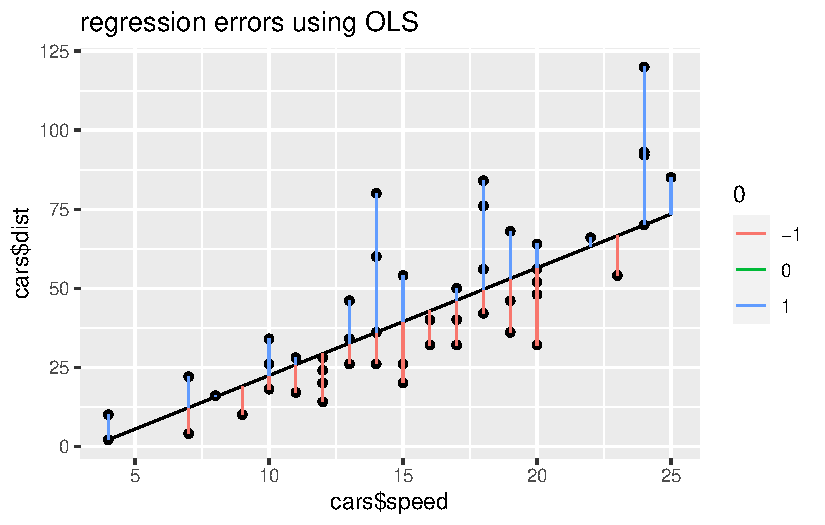
\includegraphics{methods_files/figure-pdf/unnamed-chunk-2-1.pdf}

}

\end{figure}

\begin{Shaded}
\begin{Highlighting}[]
\FunctionTok{table}\NormalTok{(color)}
\end{Highlighting}
\end{Shaded}

\begin{verbatim}
color
-1  0  1 
24  3 23 
\end{verbatim}

Notice that approximately half of the distribution of the points are
above the QR line and approximately half are above the QR line. Now
let's see what happens when we look at the 90th conditional quantile.

\begin{Shaded}
\begin{Highlighting}[]
\NormalTok{rq90 }\OtherTok{\textless{}{-}} \FunctionTok{rq}\NormalTok{(dist }\SpecialCharTok{\textasciitilde{}}\NormalTok{ speed, }\AttributeTok{data=}\NormalTok{cars, }\AttributeTok{tau=}\FloatTok{0.9}\NormalTok{)}
\NormalTok{yhat}\OtherTok{\textless{}{-}}\NormalTok{rq90}\SpecialCharTok{$}\NormalTok{fitted.values}
\NormalTok{color }\OtherTok{=} \FunctionTok{sign}\NormalTok{(rq90}\SpecialCharTok{$}\NormalTok{residuals)}
\FunctionTok{qplot}\NormalTok{(}\AttributeTok{x=}\NormalTok{cars}\SpecialCharTok{$}\NormalTok{speed, }\AttributeTok{y=}\NormalTok{cars}\SpecialCharTok{$}\NormalTok{dist)}\SpecialCharTok{+}\FunctionTok{geom\_line}\NormalTok{(}\AttributeTok{y=}\NormalTok{yhat)}\SpecialCharTok{+}
       \FunctionTok{geom\_segment}\NormalTok{(}\FunctionTok{aes}\NormalTok{(}\AttributeTok{x=}\NormalTok{cars}\SpecialCharTok{$}\NormalTok{speed, }\AttributeTok{xend=}\NormalTok{cars}\SpecialCharTok{$}\NormalTok{speed, }\AttributeTok{y=}\NormalTok{cars}\SpecialCharTok{$}\NormalTok{dist, }\AttributeTok{yend=}\NormalTok{yhat, }\AttributeTok{group=}\FunctionTok{as.factor}\NormalTok{(color), }\AttributeTok{color=}\FunctionTok{as.factor}\NormalTok{(color)))}\SpecialCharTok{+}
       \FunctionTok{labs}\NormalTok{(}\AttributeTok{title=}\StringTok{"regression errors"}\NormalTok{, }\AttributeTok{color=}\NormalTok{color)}
\end{Highlighting}
\end{Shaded}

\begin{figure}[H]

{\centering 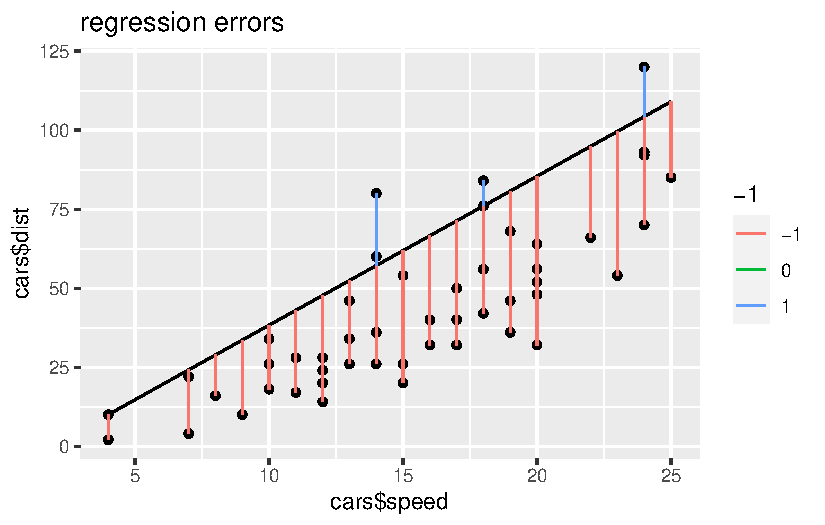
\includegraphics{methods_files/figure-pdf/unnamed-chunk-4-1.pdf}

}

\end{figure}

\begin{Shaded}
\begin{Highlighting}[]
\FunctionTok{table}\NormalTok{(color)}
\end{Highlighting}
\end{Shaded}

\begin{verbatim}
color
-1  0  1 
44  2  4 
\end{verbatim}

When we input the .9 for the quantile, we get approximately 90\% of the
points under the QR line and 10\% over the QR line.

\begin{Shaded}
\begin{Highlighting}[]
\NormalTok{rq10 }\OtherTok{\textless{}{-}} \FunctionTok{rq}\NormalTok{(dist }\SpecialCharTok{\textasciitilde{}}\NormalTok{ speed, }\AttributeTok{data=}\NormalTok{cars, }\AttributeTok{tau=}\FloatTok{0.1}\NormalTok{)}
\NormalTok{yhat}\OtherTok{\textless{}{-}}\NormalTok{rq10}\SpecialCharTok{$}\NormalTok{fitted.values}
\NormalTok{color }\OtherTok{=} \FunctionTok{sign}\NormalTok{(rq10}\SpecialCharTok{$}\NormalTok{residuals)}
\FunctionTok{qplot}\NormalTok{(}\AttributeTok{x=}\NormalTok{cars}\SpecialCharTok{$}\NormalTok{speed, }\AttributeTok{y=}\NormalTok{cars}\SpecialCharTok{$}\NormalTok{dist)}\SpecialCharTok{+}\FunctionTok{geom\_line}\NormalTok{(}\AttributeTok{y=}\NormalTok{yhat)}\SpecialCharTok{+}
       \FunctionTok{geom\_segment}\NormalTok{(}\FunctionTok{aes}\NormalTok{(}\AttributeTok{x=}\NormalTok{cars}\SpecialCharTok{$}\NormalTok{speed, }\AttributeTok{xend=}\NormalTok{cars}\SpecialCharTok{$}\NormalTok{speed, }\AttributeTok{y=}\NormalTok{cars}\SpecialCharTok{$}\NormalTok{dist, }\AttributeTok{yend=}\NormalTok{yhat, }\AttributeTok{group=}\FunctionTok{as.factor}\NormalTok{(color), }\AttributeTok{color=}\FunctionTok{as.factor}\NormalTok{(color)))}\SpecialCharTok{+}
       \FunctionTok{labs}\NormalTok{(}\AttributeTok{title=}\StringTok{"regression errors"}\NormalTok{, }\AttributeTok{color=}\NormalTok{color)}
\end{Highlighting}
\end{Shaded}

\begin{figure}[H]

{\centering 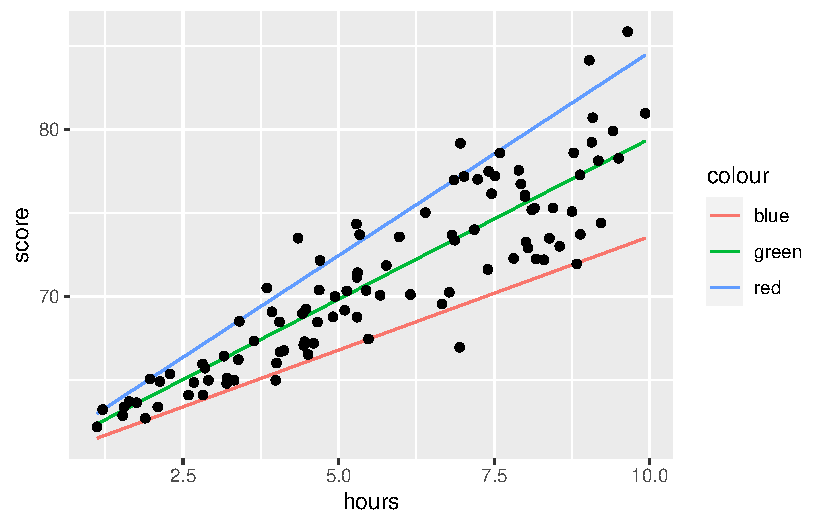
\includegraphics{methods_files/figure-pdf/unnamed-chunk-6-1.pdf}

}

\end{figure}

\begin{Shaded}
\begin{Highlighting}[]
\FunctionTok{table}\NormalTok{(color)}
\end{Highlighting}
\end{Shaded}

\begin{verbatim}
color
-1  0  1 
 5  1 44 
\end{verbatim}

When we input 0.1 for the 10th percentile, we get approximately 90\% of
the points above the QR line and 10\% below the QR line.

Thus, we can see that QR is not online a robust \#\# Evaluation metrics

\hypertarget{mean-absolute-error}{%
\subsection{Mean absolute error}\label{mean-absolute-error}}

The mean absolute error (MAE) is the average magnitude of the errors of
the values predicted by the regression and the actual observed values
for the response variable. Because it is a simple average, all errors
have the same weight, there are no penalties for different magnitude
deviations {[}2{]}. MAE assumes that the errors are normally
distributed, if the error distribution was non-normal, the average may
not be a good measure of centrality and can paint a false picture of the
goodness-of-fit of the regression curve. MAE also assumes that the
errors are unbiased. While the average magnitude of the errors is
expected to be non-zero (unless the regression is a perfect fit) the
average of the residuals, i.e., the deviation of the predicted value
from the actual value, considering underestimation and overestimation.
This means on average the regression curve does not over or
underestimate.

\[
\text { MAE }=\frac{1}{n}\sum_{i=1}^n\left|y_i-\hat{y}_i\right|=\frac{1}{n}\sum_{i=1}^n\left|e_i\right|
\]

\hypertarget{root-mean-squared-error}{%
\subsection{Root mean squared error}\label{root-mean-squared-error}}

It calculates the differences between the predictions and the actual
observations (residuals) and then gets their quadratic mean for each.
This type of error gives a larger penalty for larger errors {[}2{]}.
This error also assumes that the errors are unbiased and that they
follow a normal distribution. This gives a picture of the size of
residuals in comparison to the regression line.

\[
\operatorname{RMSE}=\sqrt{\operatorname{MSE}}=\sqrt{\frac{1}{n}\sum_{i=1}^n (y_i-\hat{y}_i)^2}=\sqrt{\frac{1}{n}\sum_{i=1}^n e_i^2}
\]

\hypertarget{variance-of-error}{%
\subsection{Variance of error}\label{variance-of-error}}

It is a measure of how spread all the errors are from the mean of all
errors.

\[
\operatorname{Var}(e)=\frac{1}{n}\sum_{i=1}^n(e_i-\bar{e})^2
\]

\hypertarget{minmax-error}{%
\subsection{Min/max error}\label{minmax-error}}

A measure of the maximum residual for a prediction and the minimum
residual.

\[
f: X \rightarrow \mathbb{R} \text {, if }(\forall e \in X_{error}) f\left(e_i\right) \geq f(e)
\]

\[
f: X \rightarrow \mathbb{R} \text {, if }(\forall e \in X_{error}) f\left(e_i\right) \leq f(e)
\]

\bookmarksetup{startatroot}

\hypertarget{analysis}{%
\chapter{Analysis}\label{analysis}}

In this analysis we aim to show that QR can achieve similar, if not
better, performance to OLS across various metrics. In order to make the
comparisons fair, we will compare the 50th quantile QR, which
corresponds to the median, to OLS regression as both the median and mean
are measures of centrality. The power of QR is that it is able to
produce similar results to OLS regression without having to meet the
strict assumptions of OLS such as the assumption of normality. In fact,
in this data set neither the response variable or predictor variables
meet the assumptions of OLS, and therefore regardless of the performance
of OLS it is invalid.

\hypertarget{visualization}{%
\section{Visualization}\label{visualization}}

\begin{Shaded}
\begin{Highlighting}[]
\NormalTok{df }\OtherTok{\textless{}{-}} \FunctionTok{read.csv}\NormalTok{(}\StringTok{"TrainData.csv"}\NormalTok{) }\SpecialCharTok{|\textgreater{}}
  \FunctionTok{na.omit}\NormalTok{() }\SpecialCharTok{|\textgreater{}}
  \FunctionTok{distinct}\NormalTok{()}
\end{Highlighting}
\end{Shaded}

\hypertarget{visualizing-data}{%
\subsection{Visualizing data}\label{visualizing-data}}

There are many different kinds of predictor variables in this data set.
For instance, there are continuous variables like GrLivArea,
discrete/coutning variables likr YearBuilt, and categorical variables
like HouseStyle. In all cases we cases we can see that the data is not
normally distributed, including in the response variable, SalePrice.
Thus, the assumptions of OLS are not met so it cannot be used to make
predictions on the data. However, for the purposes of comparing the
performance of OLS to QR. We will show that QR is able to give similar
results for this data set to OLS, and because it does not require the
same assumptions as OLS, one can actually use QR in practice for this
kind of data, which is more common than normally distributed data in
many important fields, like finance and epidemiology.

\begin{Shaded}
\begin{Highlighting}[]
\FunctionTok{suppressWarnings}\NormalTok{(\{}

\NormalTok{p1 }\OtherTok{\textless{}{-}}\NormalTok{ df }\SpecialCharTok{|\textgreater{}} \FunctionTok{ggplot}\NormalTok{(}\FunctionTok{aes}\NormalTok{(}\AttributeTok{x =}\NormalTok{ GrLivArea)) }\SpecialCharTok{+}
  \FunctionTok{geom\_histogram}\NormalTok{(}\AttributeTok{binwidth =} \DecValTok{100}\NormalTok{) }\SpecialCharTok{+}
  \FunctionTok{theme\_bw}\NormalTok{() }\SpecialCharTok{+}
  \FunctionTok{ylab}\NormalTok{(}\ConstantTok{NULL}\NormalTok{) }\SpecialCharTok{+}
  \FunctionTok{xlab}\NormalTok{(}\StringTok{"Above Ground Area (sq. ft.)"}\NormalTok{)}

\NormalTok{p2 }\OtherTok{\textless{}{-}}\NormalTok{ df }\SpecialCharTok{|\textgreater{}} \FunctionTok{ggplot}\NormalTok{(}\FunctionTok{aes}\NormalTok{(}\AttributeTok{x =}\NormalTok{ YearBuilt)) }\SpecialCharTok{+}
  \FunctionTok{geom\_histogram}\NormalTok{(}\AttributeTok{binwidth =} \DecValTok{5}\NormalTok{) }\SpecialCharTok{+}
  \FunctionTok{theme\_bw}\NormalTok{() }\SpecialCharTok{+}
  \FunctionTok{ylab}\NormalTok{(}\ConstantTok{NULL}\NormalTok{) }\SpecialCharTok{+}
  \FunctionTok{xlab}\NormalTok{(}\StringTok{"Year Built"}\NormalTok{)}

\NormalTok{p3 }\OtherTok{\textless{}{-}}\NormalTok{ df }\SpecialCharTok{|\textgreater{}} \FunctionTok{ggplot}\NormalTok{(}\FunctionTok{aes}\NormalTok{(}\AttributeTok{x =}\NormalTok{ HouseStyle)) }\SpecialCharTok{+}
  \FunctionTok{geom\_histogram}\NormalTok{(}\AttributeTok{stat=}\StringTok{"count"}\NormalTok{) }\SpecialCharTok{+}
  \FunctionTok{theme\_bw}\NormalTok{() }\SpecialCharTok{+}
  \FunctionTok{theme}\NormalTok{(}\AttributeTok{axis.text.x =} \FunctionTok{element\_text}\NormalTok{(}\AttributeTok{angle =} \DecValTok{45}\NormalTok{, }\AttributeTok{hjust =} \DecValTok{1}\NormalTok{)) }\SpecialCharTok{+}
  \FunctionTok{ylab}\NormalTok{(}\ConstantTok{NULL}\NormalTok{) }\SpecialCharTok{+}
  \FunctionTok{xlab}\NormalTok{(}\StringTok{"House Style"}\NormalTok{)}

\NormalTok{p4 }\OtherTok{\textless{}{-}}\NormalTok{ df }\SpecialCharTok{|\textgreater{}} \FunctionTok{ggplot}\NormalTok{(}\FunctionTok{aes}\NormalTok{(}\AttributeTok{x =}\NormalTok{ SalePrice)) }\SpecialCharTok{+}
  \FunctionTok{geom\_histogram}\NormalTok{(}\AttributeTok{binwidth =} \DecValTok{10000}\NormalTok{) }\SpecialCharTok{+}
  \FunctionTok{theme\_bw}\NormalTok{() }\SpecialCharTok{+}
  \FunctionTok{ylab}\NormalTok{(}\ConstantTok{NULL}\NormalTok{) }\SpecialCharTok{+}
  \FunctionTok{xlab}\NormalTok{(}\StringTok{"Sale Price ($)"}\NormalTok{)}

\FunctionTok{grid.arrange}\NormalTok{(p1, p2, p3, p4, }\AttributeTok{nrow =} \DecValTok{2}\NormalTok{)}
                 
\NormalTok{\})}
\end{Highlighting}
\end{Shaded}

\begin{figure}[H]

{\centering 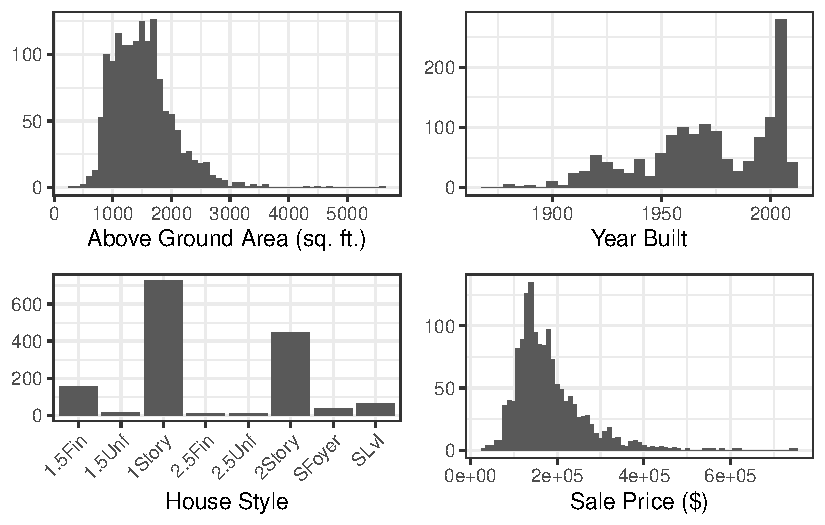
\includegraphics{analysis_files/figure-pdf/Visualizing data-1.pdf}

}

\end{figure}

\hypertarget{visualizing-quantile-regression-vs-ols}{%
\subsection{Visualizing quantile regression vs
OLS}\label{visualizing-quantile-regression-vs-ols}}

\begin{Shaded}
\begin{Highlighting}[]
\NormalTok{df }\SpecialCharTok{|\textgreater{}} \FunctionTok{ggplot}\NormalTok{(}\FunctionTok{aes}\NormalTok{(}\AttributeTok{y =}\NormalTok{ SalePrice, }\AttributeTok{x =}\NormalTok{ LotArea)) }\SpecialCharTok{+}
  \FunctionTok{geom\_point}\NormalTok{(}\AttributeTok{size =} \FloatTok{0.9}\NormalTok{) }\SpecialCharTok{+}
  \FunctionTok{geom\_smooth}\NormalTok{(}\AttributeTok{method =}\NormalTok{ lm, }\AttributeTok{se =}\NormalTok{ F, }\AttributeTok{color =} \StringTok{"black"}\NormalTok{) }\SpecialCharTok{+}
  \FunctionTok{geom\_text}\NormalTok{(}\FunctionTok{aes}\NormalTok{(}\AttributeTok{y =} \DecValTok{400000}\NormalTok{, }\AttributeTok{x =} \DecValTok{150000}\NormalTok{, }\AttributeTok{label =} \StringTok{"OLS"}\NormalTok{), }\AttributeTok{color=}\StringTok{"black"}\NormalTok{) }\SpecialCharTok{+} 
  \FunctionTok{geom\_quantile}\NormalTok{(}\AttributeTok{quantiles=}\FloatTok{0.5}\NormalTok{, }\AttributeTok{color=}\StringTok{"red"}\NormalTok{) }\SpecialCharTok{+} 
  \FunctionTok{geom\_text}\NormalTok{(}\FunctionTok{aes}\NormalTok{(}\AttributeTok{y =} \DecValTok{470000}\NormalTok{, }\AttributeTok{x =} \DecValTok{90000}\NormalTok{, }\AttributeTok{label =} \StringTok{"50th quantile"}\NormalTok{), }\AttributeTok{color=}\StringTok{"red"}\NormalTok{) }\SpecialCharTok{+} 
  \FunctionTok{ylab}\NormalTok{(}\StringTok{"Sale price ($)"}\NormalTok{) }\SpecialCharTok{+}
  \FunctionTok{xlab}\NormalTok{(}\StringTok{"Lot area (Square feet)"}\NormalTok{) }\SpecialCharTok{+}
  \FunctionTok{theme\_bw}\NormalTok{()}
\end{Highlighting}
\end{Shaded}

\begin{figure}[H]

{\centering 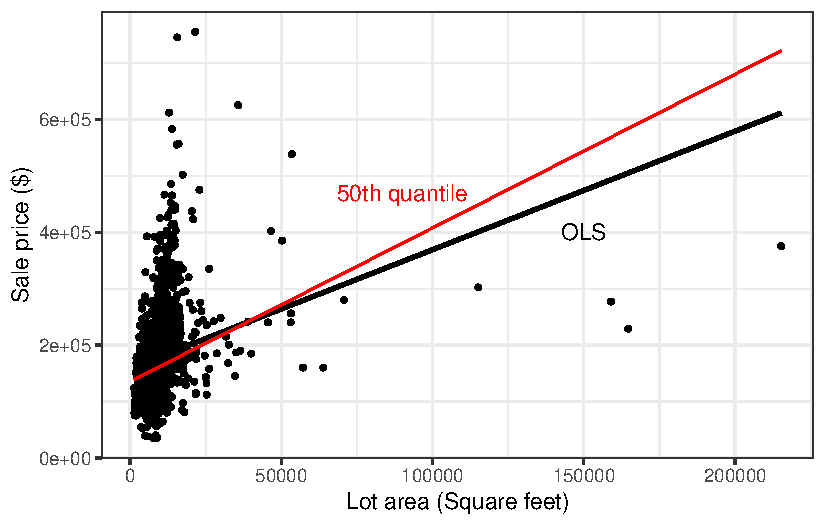
\includegraphics{analysis_files/figure-pdf/Visualizing housing-1.pdf}

}

\end{figure}

\begin{Shaded}
\begin{Highlighting}[]
\CommentTok{\# df |\textgreater{} ggplot(aes(y = SalePrice, x = GrLivArea)) +}
\CommentTok{\#   geom\_boxplot()}

\NormalTok{df }\SpecialCharTok{|\textgreater{}} \FunctionTok{ggplot}\NormalTok{(}\FunctionTok{aes}\NormalTok{(}\AttributeTok{y =}\NormalTok{ SalePrice, }\AttributeTok{x =}\NormalTok{ GrLivArea)) }\SpecialCharTok{+}
  \FunctionTok{geom\_point}\NormalTok{(}\AttributeTok{size =} \FloatTok{0.9}\NormalTok{) }\SpecialCharTok{+}
  \FunctionTok{stat\_smooth}\NormalTok{(}\AttributeTok{method =}\NormalTok{ lm, }\AttributeTok{color =} \StringTok{"black"}\NormalTok{) }\SpecialCharTok{+}
  \FunctionTok{geom\_text}\NormalTok{(}\FunctionTok{aes}\NormalTok{(}\AttributeTok{x =} \DecValTok{4150}\NormalTok{, }\AttributeTok{y =} \DecValTok{500000}\NormalTok{, }\AttributeTok{label =} \StringTok{"OLS"}\NormalTok{), }\AttributeTok{color=}\StringTok{"black"}\NormalTok{) }\SpecialCharTok{+} 
  \FunctionTok{geom\_quantile}\NormalTok{(}\AttributeTok{quantiles=}\FloatTok{0.25}\NormalTok{, }\AttributeTok{color=}\StringTok{"red"}\NormalTok{) }\SpecialCharTok{+} 
  \FunctionTok{geom\_text}\NormalTok{(}\FunctionTok{aes}\NormalTok{(}\AttributeTok{x =} \DecValTok{4000}\NormalTok{, }\AttributeTok{y =} \DecValTok{270000}\NormalTok{, }\AttributeTok{label =} \StringTok{"25th quantile"}\NormalTok{), }\AttributeTok{color=}\StringTok{"red"}\NormalTok{) }\SpecialCharTok{+} 
  \FunctionTok{geom\_quantile}\NormalTok{(}\AttributeTok{quantiles=}\FloatTok{0.5}\NormalTok{, }\AttributeTok{color=}\StringTok{"blue"}\NormalTok{) }\SpecialCharTok{+} 
  \FunctionTok{geom\_text}\NormalTok{(}\FunctionTok{aes}\NormalTok{(}\AttributeTok{x =} \DecValTok{4150}\NormalTok{, }\AttributeTok{y =} \DecValTok{400000}\NormalTok{, }\AttributeTok{label =} \StringTok{"50th"}\NormalTok{), }\AttributeTok{color=}\StringTok{"blue"}\NormalTok{) }\SpecialCharTok{+} 
  \FunctionTok{geom\_quantile}\NormalTok{(}\AttributeTok{quantiles=}\FloatTok{0.75}\NormalTok{, }\AttributeTok{color=}\StringTok{"green"}\NormalTok{) }\SpecialCharTok{+} 
  \FunctionTok{geom\_text}\NormalTok{(}\FunctionTok{aes}\NormalTok{(}\AttributeTok{x =} \DecValTok{4000}\NormalTok{, }\AttributeTok{y =} \DecValTok{600000}\NormalTok{, }\AttributeTok{label =} \StringTok{"75th quantile"}\NormalTok{), }\AttributeTok{color=}\StringTok{"green"}\NormalTok{) }\SpecialCharTok{+} 
  \FunctionTok{xlab}\NormalTok{(}\StringTok{"Sale price ($)"}\NormalTok{) }\SpecialCharTok{+}
  \FunctionTok{ylab}\NormalTok{(}\StringTok{"Above ground area (Square feet)"}\NormalTok{) }\SpecialCharTok{+}
  \FunctionTok{theme\_bw}\NormalTok{()}
\end{Highlighting}
\end{Shaded}

\begin{figure}[H]

{\centering 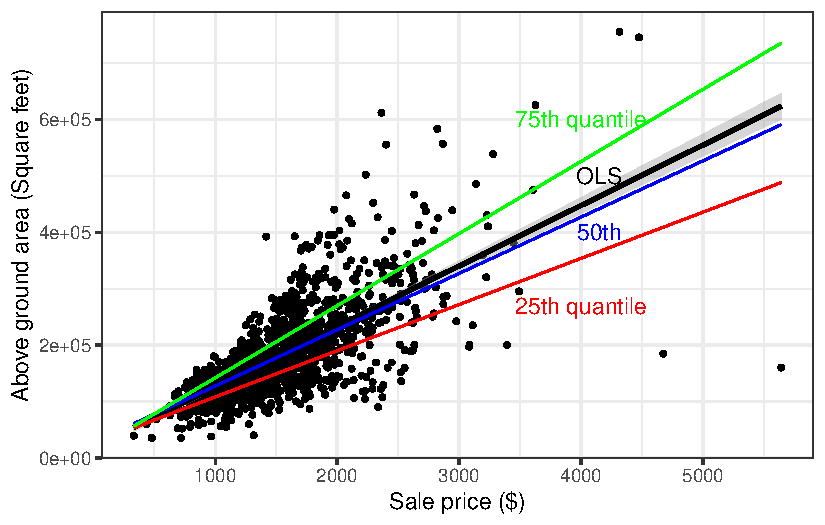
\includegraphics{analysis_files/figure-pdf/Visualizing housing-2.pdf}

}

\end{figure}

\hypertarget{model-creation}{%
\section{Model creation}\label{model-creation}}

\hypertarget{qr-model}{%
\subsection{QR model}\label{qr-model}}

\begin{Shaded}
\begin{Highlighting}[]
\NormalTok{qr50 }\OtherTok{=} \FunctionTok{rq}\NormalTok{(}\AttributeTok{data=}\NormalTok{df, SalePrice }\SpecialCharTok{\textasciitilde{}}\NormalTok{ GrLivArea }\SpecialCharTok{+}\NormalTok{ LotArea }\SpecialCharTok{+}\NormalTok{ TotRmsAbvGrd }\SpecialCharTok{+} \FunctionTok{as.factor}\NormalTok{(LotShape) }\SpecialCharTok{+} \FunctionTok{as.factor}\NormalTok{(Foundation), }\AttributeTok{tau=}\FloatTok{0.5}\NormalTok{)}
\NormalTok{qr50\_summary }\OtherTok{=} \FunctionTok{summary}\NormalTok{(qr50)}
\NormalTok{qr50\_summary}
\end{Highlighting}
\end{Shaded}

\begin{verbatim}

Call: rq(formula = SalePrice ~ GrLivArea + LotArea + TotRmsAbvGrd + 
    as.factor(LotShape) + as.factor(Foundation), tau = 0.5, data = df)

tau: [1] 0.5

Coefficients:
                            Value        Std. Error   t value      Pr(>|t|)    
(Intercept)                  36326.81296   3853.84854      9.42611      0.00000
GrLivArea                       96.66934      4.02708     24.00481      0.00000
LotArea                          0.99940      0.32815      3.04561      0.00236
TotRmsAbvGrd                 -6476.18114   1080.95132     -5.99119      0.00000
as.factor(LotShape)IR2       -5084.13375   7841.20685     -0.64839      0.51684
as.factor(LotShape)IR3      -21074.80675   7616.42154     -2.76702      0.00573
as.factor(LotShape)Reg      -11065.07360   2020.92512     -5.47525      0.00000
as.factor(Foundation)CBlock  21252.40678   1709.40460     12.43264      0.00000
as.factor(Foundation)PConc   53311.16094   2618.05941     20.36285      0.00000
as.factor(Foundation)Slab   -16867.20619   5378.30454     -3.13616      0.00175
as.factor(Foundation)Stone   14561.54748  13561.64146      1.07373      0.28312
as.factor(Foundation)Wood    -2008.81877   9022.14216     -0.22265      0.82384
\end{verbatim}

\hypertarget{ols-model}{%
\subsection{OLS model}\label{ols-model}}

\begin{Shaded}
\begin{Highlighting}[]
\NormalTok{ols }\OtherTok{=} \FunctionTok{lm}\NormalTok{(}\AttributeTok{data=}\NormalTok{df, SalePrice }\SpecialCharTok{\textasciitilde{}}\NormalTok{ GrLivArea }\SpecialCharTok{+}\NormalTok{ LotArea }\SpecialCharTok{+}\NormalTok{ TotRmsAbvGrd }\SpecialCharTok{+} \FunctionTok{as.factor}\NormalTok{(LotShape) }\SpecialCharTok{+} \FunctionTok{as.factor}\NormalTok{(Foundation))}
\NormalTok{ols\_summary }\OtherTok{=} \FunctionTok{summary}\NormalTok{(ols)}
\NormalTok{ols\_summary}
\end{Highlighting}
\end{Shaded}

\begin{verbatim}

Call:
lm(formula = SalePrice ~ GrLivArea + LotArea + TotRmsAbvGrd + 
    as.factor(LotShape) + as.factor(Foundation), data = df)

Residuals:
    Min      1Q  Median      3Q     Max 
-422488  -26194    -805   20461  326538 

Coefficients:
                              Estimate Std. Error t value Pr(>|t|)    
(Intercept)                  2.005e+04  7.267e+03   2.759  0.00587 ** 
GrLivArea                    9.893e+01  4.538e+00  21.801  < 2e-16 ***
LotArea                      9.173e-01  1.425e-01   6.438 1.64e-10 ***
TotRmsAbvGrd                -4.313e+03  1.396e+03  -3.089  0.00205 ** 
as.factor(LotShape)IR2      -2.009e+03  8.113e+03  -0.248  0.80446    
as.factor(LotShape)IR3      -6.936e+04  1.603e+04  -4.328 1.61e-05 ***
as.factor(LotShape)Reg      -1.342e+04  2.809e+03  -4.777 1.96e-06 ***
as.factor(Foundation)CBlock  2.094e+04  4.497e+03   4.656 3.52e-06 ***
as.factor(Foundation)PConc   6.679e+04  4.541e+03  14.708  < 2e-16 ***
as.factor(Foundation)Slab   -1.426e+04  1.067e+04  -1.336  0.18170    
as.factor(Foundation)Stone  -3.396e+03  2.021e+04  -0.168  0.86658    
as.factor(Foundation)Wood   -5.553e+02  2.842e+04  -0.020  0.98441    
---
Signif. codes:  0 '***' 0.001 '**' 0.01 '*' 0.05 '.' 0.1 ' ' 1

Residual standard error: 48410 on 1448 degrees of freedom
Multiple R-squared:  0.6315,    Adjusted R-squared:  0.6287 
F-statistic: 225.6 on 11 and 1448 DF,  p-value: < 2.2e-16
\end{verbatim}

\hypertarget{model-evaluation}{%
\section{Model evaluation}\label{model-evaluation}}

\hypertarget{mean-absolute-error-1}{%
\subsection{Mean absolute error}\label{mean-absolute-error-1}}

\begin{Shaded}
\begin{Highlighting}[]
\NormalTok{olsMae }\OtherTok{=} \FunctionTok{mae}\NormalTok{(}\FunctionTok{predict}\NormalTok{(ols), df}\SpecialCharTok{$}\NormalTok{SalePrice)}
\NormalTok{olsMae}
\end{Highlighting}
\end{Shaded}

\begin{verbatim}
[1] 32186.89
\end{verbatim}

\begin{Shaded}
\begin{Highlighting}[]
\NormalTok{Qr50Mae }\OtherTok{=} \FunctionTok{mae}\NormalTok{(}\FunctionTok{predict}\NormalTok{(qr50), df}\SpecialCharTok{$}\NormalTok{SalePrice)}
\NormalTok{Qr50Mae}
\end{Highlighting}
\end{Shaded}

\begin{verbatim}
[1] 31160.69
\end{verbatim}

OLS MAE value: 32186.89.

And QR 50th MAE value: 31160.69.

QR for 50th quantile has a lower MAE therefore it is has more accurate
predictions.

\hypertarget{root-mean-squared-error-1}{%
\subsection{Root mean squared error}\label{root-mean-squared-error-1}}

\begin{Shaded}
\begin{Highlighting}[]
\NormalTok{olsRmse }\OtherTok{=} \FunctionTok{rmse}\NormalTok{(}\FunctionTok{predict}\NormalTok{(ols), df}\SpecialCharTok{$}\NormalTok{SalePrice)}
\NormalTok{olsRmse}
\end{Highlighting}
\end{Shaded}

\begin{verbatim}
[1] 48209.34
\end{verbatim}

\begin{Shaded}
\begin{Highlighting}[]
\NormalTok{Qr50Rmse }\OtherTok{=} \FunctionTok{rmse}\NormalTok{(}\FunctionTok{predict}\NormalTok{(qr50), df}\SpecialCharTok{$}\NormalTok{SalePrice)}
\NormalTok{Qr50Rmse}
\end{Highlighting}
\end{Shaded}

\begin{verbatim}
[1] 49434.81
\end{verbatim}

OLS RMSE value: 48209.34.

And QR 50th RMSE value: 49434.81.

Since OLS algorithm's goal is to minimize RMSE, as expected it has a
better (lower) value. But QR has a very similar value which shows how
well QR model can keep up even if it is not focusing on optimizing RMSE.

\hypertarget{variance-of-error-1}{%
\subsection{Variance of error}\label{variance-of-error-1}}

\begin{Shaded}
\begin{Highlighting}[]
\NormalTok{ols\_summary}\SpecialCharTok{$}\NormalTok{df[}\DecValTok{2}\NormalTok{]}
\end{Highlighting}
\end{Shaded}

\begin{verbatim}
[1] 1448
\end{verbatim}

\begin{Shaded}
\begin{Highlighting}[]
\NormalTok{qr50\_summary}\SpecialCharTok{$}\NormalTok{rdf}
\end{Highlighting}
\end{Shaded}

\begin{verbatim}
[1] 1448
\end{verbatim}

The variance of error for OLS: 1448.

The variance of error for QR 50th: 1448.

Both have the same variance of error.

\hypertarget{minmax-error-1}{%
\subsection{Min/max error}\label{minmax-error-1}}

\begin{Shaded}
\begin{Highlighting}[]
\CommentTok{\# Min OLS error}
\FunctionTok{format}\NormalTok{(}\FunctionTok{round}\NormalTok{(}\FunctionTok{min}\NormalTok{(ols\_summary}\SpecialCharTok{$}\NormalTok{residuals), }\AttributeTok{digits=}\DecValTok{0}\NormalTok{), }\AttributeTok{scientific=}\NormalTok{F)}
\end{Highlighting}
\end{Shaded}

\begin{verbatim}
[1] "-422488"
\end{verbatim}

\begin{Shaded}
\begin{Highlighting}[]
\CommentTok{\# Absolute min OLS error}
\FunctionTok{format}\NormalTok{(}\FunctionTok{round}\NormalTok{(}\FunctionTok{min}\NormalTok{(}\FunctionTok{abs}\NormalTok{(ols\_summary}\SpecialCharTok{$}\NormalTok{residuals)), }\AttributeTok{digits=}\DecValTok{0}\NormalTok{), }\AttributeTok{scientific=}\NormalTok{F)}
\end{Highlighting}
\end{Shaded}

\begin{verbatim}
[1] "5"
\end{verbatim}

\begin{Shaded}
\begin{Highlighting}[]
\CommentTok{\# Max OLS error}
\FunctionTok{format}\NormalTok{(}\FunctionTok{round}\NormalTok{(}\FunctionTok{max}\NormalTok{(ols\_summary}\SpecialCharTok{$}\NormalTok{residuals), }\AttributeTok{digits=}\DecValTok{0}\NormalTok{), }\AttributeTok{scientific=}\NormalTok{F)}
\end{Highlighting}
\end{Shaded}

\begin{verbatim}
[1] "326538"
\end{verbatim}

\begin{Shaded}
\begin{Highlighting}[]
\CommentTok{\# Absolute max OLS error}
\FunctionTok{format}\NormalTok{(}\FunctionTok{round}\NormalTok{(}\FunctionTok{max}\NormalTok{(}\FunctionTok{abs}\NormalTok{(ols\_summary}\SpecialCharTok{$}\NormalTok{residuals)), }\AttributeTok{digits=}\DecValTok{0}\NormalTok{), }\AttributeTok{scientific=}\NormalTok{F)}
\end{Highlighting}
\end{Shaded}

\begin{verbatim}
[1] "422488"
\end{verbatim}

\begin{Shaded}
\begin{Highlighting}[]
\CommentTok{\# Min QR 50th error}
\FunctionTok{format}\NormalTok{(}\FunctionTok{round}\NormalTok{(}\FunctionTok{min}\NormalTok{(qr50\_summary}\SpecialCharTok{$}\NormalTok{residuals), }\AttributeTok{digits=}\DecValTok{0}\NormalTok{), }\AttributeTok{scientific=}\NormalTok{F)}
\end{Highlighting}
\end{Shaded}

\begin{verbatim}
[1] "-440106"
\end{verbatim}

\begin{Shaded}
\begin{Highlighting}[]
\CommentTok{\# Absolute min QR 50th error}
\FunctionTok{format}\NormalTok{(}\FunctionTok{round}\NormalTok{(}\FunctionTok{min}\NormalTok{(}\FunctionTok{abs}\NormalTok{(qr50\_summary}\SpecialCharTok{$}\NormalTok{residuals)), }\AttributeTok{digits=}\DecValTok{0}\NormalTok{), }\AttributeTok{scientific=}\NormalTok{F)}
\end{Highlighting}
\end{Shaded}

\begin{verbatim}
[1] "0"
\end{verbatim}

\begin{Shaded}
\begin{Highlighting}[]
\CommentTok{\# Max QR 50th error}
\FunctionTok{format}\NormalTok{(}\FunctionTok{round}\NormalTok{(}\FunctionTok{max}\NormalTok{(qr50\_summary}\SpecialCharTok{$}\NormalTok{residuals), }\AttributeTok{digits=}\DecValTok{0}\NormalTok{), }\AttributeTok{scientific=}\NormalTok{F)}
\end{Highlighting}
\end{Shaded}

\begin{verbatim}
[1] "351819"
\end{verbatim}

\begin{Shaded}
\begin{Highlighting}[]
\CommentTok{\# Absolute max QR 50th error}
\FunctionTok{format}\NormalTok{(}\FunctionTok{round}\NormalTok{(}\FunctionTok{max}\NormalTok{(}\FunctionTok{abs}\NormalTok{(qr50\_summary}\SpecialCharTok{$}\NormalTok{residuals)), }\AttributeTok{digits=}\DecValTok{0}\NormalTok{), }\AttributeTok{scientific=}\NormalTok{F)}
\end{Highlighting}
\end{Shaded}

\begin{verbatim}
[1] "440106"
\end{verbatim}

\hypertarget{ols}{%
\subsubsection{OLS}\label{ols}}

Min OLS error: -422488.

Absolute min OLS error: 5.

Max OLS error: 326538.

Absolute max OLS error: 422488.

\hypertarget{qr}{%
\subsubsection{QR}\label{qr}}

Min QR 50th error: -440106.

Absolute min QR 50th error: 0.

Max QR 50th error: 351819.

Absolute max QR 50th error: 440106.

\bookmarksetup{startatroot}

\hypertarget{summary}{%
\chapter{Summary}\label{summary}}

In summary, this book has no content whatsoever.

\begin{Shaded}
\begin{Highlighting}[]
\DecValTok{1} \SpecialCharTok{+} \DecValTok{1}
\end{Highlighting}
\end{Shaded}

\begin{verbatim}
[1] 2
\end{verbatim}

\bookmarksetup{startatroot}

\hypertarget{references}{%
\chapter*{References}\label{references}}
\addcontentsline{toc}{chapter}{References}

\markboth{References}{References}

{[}1{]} R. Koenker and G. Bassett Jr, ``REGRESSION QUANTILES,''
Econometrica (Pre-1986), vol.~46, (1), pp.~33, 1978. Available:
https://login.lp.hscl.ufl.edu/login?url=https://www.proquest.com/scholarly-journals/regression-quantiles/docview/214661061/se-2.

\noindent [2] Chai, T., \& Draxler, R. R. (2014). Root mean square error
(RMSE) or mean absolute error (MAE)? - Arguments against avoiding RMSE
in the literature. Geoscientific Model Development, 7(3), 1247.
https://link-gale-com.ezproxy.lib.uwf.edu/apps/doc/A481458766/AONE?u=pens49866\&sid=bookmark-AONE\&xid=4c31b5f6

\hypertarget{refs}{}
\begin{CSLReferences}{0}{0}
\end{CSLReferences}



\end{document}
